% Options for packages loaded elsewhere
% Options for packages loaded elsewhere
\PassOptionsToPackage{unicode}{hyperref}
\PassOptionsToPackage{hyphens}{url}
\PassOptionsToPackage{dvipsnames,svgnames,x11names}{xcolor}
%
\documentclass[
  spanish,
  11pt,
  a4paper,
  DIV=11,
  numbers=noendperiod]{scrartcl}
\usepackage{xcolor}
\usepackage[margin=2.5cm]{geometry}
\usepackage{amsmath,amssymb}
\setcounter{secnumdepth}{5}
\usepackage{iftex}
\ifPDFTeX
  \usepackage[T1]{fontenc}
  \usepackage[utf8]{inputenc}
  \usepackage{textcomp} % provide euro and other symbols
\else % if luatex or xetex
  \usepackage{unicode-math} % this also loads fontspec
  \defaultfontfeatures{Scale=MatchLowercase}
  \defaultfontfeatures[\rmfamily]{Ligatures=TeX,Scale=1}
\fi
\usepackage{lmodern}
\ifPDFTeX\else
  % xetex/luatex font selection
  \setmainfont[]{Times New Roman}
\fi
% Use upquote if available, for straight quotes in verbatim environments
\IfFileExists{upquote.sty}{\usepackage{upquote}}{}
\IfFileExists{microtype.sty}{% use microtype if available
  \usepackage[]{microtype}
  \UseMicrotypeSet[protrusion]{basicmath} % disable protrusion for tt fonts
}{}
\makeatletter
\@ifundefined{KOMAClassName}{% if non-KOMA class
  \IfFileExists{parskip.sty}{%
    \usepackage{parskip}
  }{% else
    \setlength{\parindent}{0pt}
    \setlength{\parskip}{6pt plus 2pt minus 1pt}}
}{% if KOMA class
  \KOMAoptions{parskip=half}}
\makeatother
% Make \paragraph and \subparagraph free-standing
\makeatletter
\ifx\paragraph\undefined\else
  \let\oldparagraph\paragraph
  \renewcommand{\paragraph}{
    \@ifstar
      \xxxParagraphStar
      \xxxParagraphNoStar
  }
  \newcommand{\xxxParagraphStar}[1]{\oldparagraph*{#1}\mbox{}}
  \newcommand{\xxxParagraphNoStar}[1]{\oldparagraph{#1}\mbox{}}
\fi
\ifx\subparagraph\undefined\else
  \let\oldsubparagraph\subparagraph
  \renewcommand{\subparagraph}{
    \@ifstar
      \xxxSubParagraphStar
      \xxxSubParagraphNoStar
  }
  \newcommand{\xxxSubParagraphStar}[1]{\oldsubparagraph*{#1}\mbox{}}
  \newcommand{\xxxSubParagraphNoStar}[1]{\oldsubparagraph{#1}\mbox{}}
\fi
\makeatother

\usepackage{color}
\usepackage{fancyvrb}
\newcommand{\VerbBar}{|}
\newcommand{\VERB}{\Verb[commandchars=\\\{\}]}
\DefineVerbatimEnvironment{Highlighting}{Verbatim}{commandchars=\\\{\}}
% Add ',fontsize=\small' for more characters per line
\usepackage{framed}
\definecolor{shadecolor}{RGB}{241,243,245}
\newenvironment{Shaded}{\begin{snugshade}}{\end{snugshade}}
\newcommand{\AlertTok}[1]{\textcolor[rgb]{0.68,0.00,0.00}{#1}}
\newcommand{\AnnotationTok}[1]{\textcolor[rgb]{0.37,0.37,0.37}{#1}}
\newcommand{\AttributeTok}[1]{\textcolor[rgb]{0.40,0.45,0.13}{#1}}
\newcommand{\BaseNTok}[1]{\textcolor[rgb]{0.68,0.00,0.00}{#1}}
\newcommand{\BuiltInTok}[1]{\textcolor[rgb]{0.00,0.23,0.31}{#1}}
\newcommand{\CharTok}[1]{\textcolor[rgb]{0.13,0.47,0.30}{#1}}
\newcommand{\CommentTok}[1]{\textcolor[rgb]{0.37,0.37,0.37}{#1}}
\newcommand{\CommentVarTok}[1]{\textcolor[rgb]{0.37,0.37,0.37}{\textit{#1}}}
\newcommand{\ConstantTok}[1]{\textcolor[rgb]{0.56,0.35,0.01}{#1}}
\newcommand{\ControlFlowTok}[1]{\textcolor[rgb]{0.00,0.23,0.31}{\textbf{#1}}}
\newcommand{\DataTypeTok}[1]{\textcolor[rgb]{0.68,0.00,0.00}{#1}}
\newcommand{\DecValTok}[1]{\textcolor[rgb]{0.68,0.00,0.00}{#1}}
\newcommand{\DocumentationTok}[1]{\textcolor[rgb]{0.37,0.37,0.37}{\textit{#1}}}
\newcommand{\ErrorTok}[1]{\textcolor[rgb]{0.68,0.00,0.00}{#1}}
\newcommand{\ExtensionTok}[1]{\textcolor[rgb]{0.00,0.23,0.31}{#1}}
\newcommand{\FloatTok}[1]{\textcolor[rgb]{0.68,0.00,0.00}{#1}}
\newcommand{\FunctionTok}[1]{\textcolor[rgb]{0.28,0.35,0.67}{#1}}
\newcommand{\ImportTok}[1]{\textcolor[rgb]{0.00,0.46,0.62}{#1}}
\newcommand{\InformationTok}[1]{\textcolor[rgb]{0.37,0.37,0.37}{#1}}
\newcommand{\KeywordTok}[1]{\textcolor[rgb]{0.00,0.23,0.31}{\textbf{#1}}}
\newcommand{\NormalTok}[1]{\textcolor[rgb]{0.00,0.23,0.31}{#1}}
\newcommand{\OperatorTok}[1]{\textcolor[rgb]{0.37,0.37,0.37}{#1}}
\newcommand{\OtherTok}[1]{\textcolor[rgb]{0.00,0.23,0.31}{#1}}
\newcommand{\PreprocessorTok}[1]{\textcolor[rgb]{0.68,0.00,0.00}{#1}}
\newcommand{\RegionMarkerTok}[1]{\textcolor[rgb]{0.00,0.23,0.31}{#1}}
\newcommand{\SpecialCharTok}[1]{\textcolor[rgb]{0.37,0.37,0.37}{#1}}
\newcommand{\SpecialStringTok}[1]{\textcolor[rgb]{0.13,0.47,0.30}{#1}}
\newcommand{\StringTok}[1]{\textcolor[rgb]{0.13,0.47,0.30}{#1}}
\newcommand{\VariableTok}[1]{\textcolor[rgb]{0.07,0.07,0.07}{#1}}
\newcommand{\VerbatimStringTok}[1]{\textcolor[rgb]{0.13,0.47,0.30}{#1}}
\newcommand{\WarningTok}[1]{\textcolor[rgb]{0.37,0.37,0.37}{\textit{#1}}}

\usepackage{longtable,booktabs,array}
\usepackage{calc} % for calculating minipage widths
% Correct order of tables after \paragraph or \subparagraph
\usepackage{etoolbox}
\makeatletter
\patchcmd\longtable{\par}{\if@noskipsec\mbox{}\fi\par}{}{}
\makeatother
% Allow footnotes in longtable head/foot
\IfFileExists{footnotehyper.sty}{\usepackage{footnotehyper}}{\usepackage{footnote}}
\makesavenoteenv{longtable}
\usepackage{graphicx}
\makeatletter
\newsavebox\pandoc@box
\newcommand*\pandocbounded[1]{% scales image to fit in text height/width
  \sbox\pandoc@box{#1}%
  \Gscale@div\@tempa{\textheight}{\dimexpr\ht\pandoc@box+\dp\pandoc@box\relax}%
  \Gscale@div\@tempb{\linewidth}{\wd\pandoc@box}%
  \ifdim\@tempb\p@<\@tempa\p@\let\@tempa\@tempb\fi% select the smaller of both
  \ifdim\@tempa\p@<\p@\scalebox{\@tempa}{\usebox\pandoc@box}%
  \else\usebox{\pandoc@box}%
  \fi%
}
% Set default figure placement to htbp
\def\fps@figure{htbp}
\makeatother



\ifLuaTeX
\usepackage[bidi=basic]{babel}
\else
\usepackage[bidi=default]{babel}
\fi
\ifPDFTeX
\else
\babelfont{rm}[]{Times New Roman}
\fi
% get rid of language-specific shorthands (see #6817):
\let\LanguageShortHands\languageshorthands
\def\languageshorthands#1{}


\setlength{\emergencystretch}{3em} % prevent overfull lines

\providecommand{\tightlist}{%
  \setlength{\itemsep}{0pt}\setlength{\parskip}{0pt}}



 


\KOMAoption{captions}{tableheading}
\makeatletter
\@ifpackageloaded{caption}{}{\usepackage{caption}}
\AtBeginDocument{%
\ifdefined\contentsname
  \renewcommand*\contentsname{Tabla de contenidos}
\else
  \newcommand\contentsname{Tabla de contenidos}
\fi
\ifdefined\listfigurename
  \renewcommand*\listfigurename{Listado de Figuras}
\else
  \newcommand\listfigurename{Listado de Figuras}
\fi
\ifdefined\listtablename
  \renewcommand*\listtablename{Listado de Tablas}
\else
  \newcommand\listtablename{Listado de Tablas}
\fi
\ifdefined\figurename
  \renewcommand*\figurename{Figura}
\else
  \newcommand\figurename{Figura}
\fi
\ifdefined\tablename
  \renewcommand*\tablename{Tabla}
\else
  \newcommand\tablename{Tabla}
\fi
}
\@ifpackageloaded{float}{}{\usepackage{float}}
\floatstyle{ruled}
\@ifundefined{c@chapter}{\newfloat{codelisting}{h}{lop}}{\newfloat{codelisting}{h}{lop}[chapter]}
\floatname{codelisting}{Listado}
\newcommand*\listoflistings{\listof{codelisting}{Listado de Listados}}
\makeatother
\makeatletter
\makeatother
\makeatletter
\@ifpackageloaded{caption}{}{\usepackage{caption}}
\@ifpackageloaded{subcaption}{}{\usepackage{subcaption}}
\makeatother
\usepackage{bookmark}
\IfFileExists{xurl.sty}{\usepackage{xurl}}{} % add URL line breaks if available
\urlstyle{same}
\hypersetup{
  pdftitle={Prueba de hipótesis},
  pdfauthor={Santos G},
  pdflang={es},
  colorlinks=true,
  linkcolor={blue},
  filecolor={Maroon},
  citecolor={Blue},
  urlcolor={Blue},
  pdfcreator={LaTeX via pandoc}}


\title{Prueba de hipótesis}
\author{Santos G}
\date{}
\begin{document}
\maketitle

\renewcommand*\contentsname{Tabla de contenidos}
{
\hypersetup{linkcolor=}
\setcounter{tocdepth}{2}
\tableofcontents
}

\section{Contexto del proyecto}\label{contexto-del-proyecto}

El estudio de diferencias morfométricas entre especies es fundamental
para comprender las adaptaciones ecológicas que presentan los organismos
en relación con su ambiente y dieta. En el caso de los pingüinos de la
Antártida, variables como el largo del pico permiten explorar cómo cada
especie se especializa en la captura de presas y la ocupación de
distintos nichos tróficos.

En este análisis trabajaremos con el dataset \texttt{palmerpenguins},
que contiene información morfométrica de tres especies (\emph{Adelie,
Chinstrap y Gentoo}). Previamente, los datos fueron limpiados y
verificados, de modo que ahora podemos avanzar hacia las pruebas
estadísticas que comparan medias entre grupos.

\textbf{Pregunta de investigación:}\\
¿Existen diferencias significativas en el largo del pico
(\emph{bill\_length\_mm}) entre las tres especies de pingüinos?

\section{Carga de líbrerías y
datos}\label{carga-de-luxedbreruxedas-y-datos}

\begin{Shaded}
\begin{Highlighting}[numbers=left,,]
\CommentTok{\#|label: prep}
\FunctionTok{library}\NormalTok{(tidyverse)   }\CommentTok{\# dplyr, ggplot2, tidyr: manipulación de datos y gráficos}
\FunctionTok{library}\NormalTok{(janitor)     }\CommentTok{\# clean\_names(): estandarizar nombres de variables}
\FunctionTok{library}\NormalTok{(palmerpenguins) }\CommentTok{\# dataset de ejemplo (penguins)}
\FunctionTok{library}\NormalTok{(car)         }\CommentTok{\# leveneTest(): prueba de homogeneidad de varianzas}
\FunctionTok{library}\NormalTok{(rstatix)     }\CommentTok{\# funciones rápidas para ANOVA, Kruskal–Wallis, post{-}hoc}
\FunctionTok{library}\NormalTok{(ggpubr)      }\CommentTok{\# visualización de resultados estadísticos}

\NormalTok{df\_raw }\OtherTok{\textless{}{-}}\NormalTok{ penguins }\SpecialCharTok{\%\textgreater{}\%} \FunctionTok{as\_tibble}\NormalTok{() }\CommentTok{\# guardo raw para auditoría}
\NormalTok{df }\OtherTok{\textless{}{-}}\NormalTok{ df\_raw }\SpecialCharTok{\%\textgreater{}\%} \FunctionTok{clean\_names}\NormalTok{()}
\end{Highlighting}
\end{Shaded}

\section{Verificación de supuestos}\label{verificaciuxf3n-de-supuestos}

\begin{Shaded}
\begin{Highlighting}[numbers=left,,]
\NormalTok{modelo }\OtherTok{\textless{}{-}} \FunctionTok{aov}\NormalTok{(bill\_length\_mm }\SpecialCharTok{\textasciitilde{}}\NormalTok{ species, }\AttributeTok{data =}\NormalTok{ df)                                  }

\CommentTok{\# Normalidad de residuos}
\NormalTok{Normalidad }\OtherTok{\textless{}{-}} \FunctionTok{shapiro.test}\NormalTok{(}\FunctionTok{residuals}\NormalTok{(modelo))}

\CommentTok{\# Homogeneidad de varianzas (Levene)}
\NormalTok{Homogeneidad }\OtherTok{\textless{}{-}} \FunctionTok{leveneTest}\NormalTok{(bill\_length\_mm }\SpecialCharTok{\textasciitilde{}}\NormalTok{ species, }\AttributeTok{data =}\NormalTok{ df)}

\CommentTok{\# Tablas}
\NormalTok{knitr}\SpecialCharTok{::}\FunctionTok{kable}\NormalTok{(}
\NormalTok{  broom}\SpecialCharTok{::}\FunctionTok{tidy}\NormalTok{(Normalidad),}
  \AttributeTok{caption =} \StringTok{"Test de normalidad de residuos (Shapiro{-}Wilk)"}
\NormalTok{)}
\end{Highlighting}
\end{Shaded}

\begin{longtable}[]{@{}rrl@{}}
\caption{Test de normalidad de residuos (Shapiro-Wilk)}\tabularnewline
\toprule\noalign{}
statistic & p.value & method \\
\midrule\noalign{}
\endfirsthead
\toprule\noalign{}
statistic & p.value & method \\
\midrule\noalign{}
\endhead
\bottomrule\noalign{}
\endlastfoot
0.9890313 & 0.0113053 & Shapiro-Wilk normality test \\
\end{longtable}

\begin{Shaded}
\begin{Highlighting}[numbers=left,,]
\NormalTok{knitr}\SpecialCharTok{::}\FunctionTok{kable}\NormalTok{(}
\NormalTok{  broom}\SpecialCharTok{::}\FunctionTok{tidy}\NormalTok{(Homogeneidad),}
  \AttributeTok{caption =} \StringTok{"Test de homogeneidad de varianzas (Levene)"}
\NormalTok{)}
\end{Highlighting}
\end{Shaded}

\begin{longtable}[]{@{}rrrr@{}}
\caption{Test de homogeneidad de varianzas (Levene)}\tabularnewline
\toprule\noalign{}
statistic & p.value & df & df.residual \\
\midrule\noalign{}
\endfirsthead
\toprule\noalign{}
statistic & p.value & df & df.residual \\
\midrule\noalign{}
\endhead
\bottomrule\noalign{}
\endlastfoot
2.242456 & 0.1077705 & 2 & 339 \\
\end{longtable}

En la \textbf{Tabla 1} se presentan los resultados del test
Shapiro--Wilk ( W = 0.989, p = 0.0113 ). el valor p es menor a 0.05; por
lo tanto, se rechaza la normalidad de los residuos. En cuanto a la
homogeneidad de varianzas, en la \textbf{Tabla 2} se reflejan los
resultados del test de Levene (F = 2.242, p = 0.108 ) arrojó un valor p
mayor a 0.05, lo que indica que no se rechaza este supuesto, es decir
las varianzas entre grupos pueden considerarse similares.

En consecuencia, dado que el supuesto de normalidad no se cumple, aunque
sí el de homogeneidad de varianzas, la opción más segura y robusta es
realizar Kruskal--Wallis (prueba no paramétrica).

\section{Ejeccución del Kruskal-Wallis
global}\label{ejeccuciuxf3n-del-kruskal-wallis-global}

\begin{Shaded}
\begin{Highlighting}[numbers=left,,]
\CommentTok{\#|label: kruskal\_global}

\CommentTok{\# Kruskal{-}Wallis (global)}
\NormalTok{kruskal\_res }\OtherTok{\textless{}{-}}\NormalTok{ df }\SpecialCharTok{\%\textgreater{}\%} \FunctionTok{kruskal\_test}\NormalTok{(bill\_length\_mm }\SpecialCharTok{\textasciitilde{}}\NormalTok{ species)}

\CommentTok{\# Formatear p{-}value como p \textless{} 0.001 si es muy pequeño}
\NormalTok{kruskal\_res }\OtherTok{\textless{}{-}}\NormalTok{ kruskal\_res }\SpecialCharTok{\%\textgreater{}\%}
  \FunctionTok{mutate}\NormalTok{(}\AttributeTok{p =} \FunctionTok{ifelse}\NormalTok{(p }\SpecialCharTok{\textless{}} \FloatTok{0.001}\NormalTok{, }\StringTok{"\textless{} 0.001"}\NormalTok{, }\FunctionTok{round}\NormalTok{(p, }\DecValTok{3}\NormalTok{)))}

\NormalTok{knitr}\SpecialCharTok{::}\FunctionTok{kable}\NormalTok{(kruskal\_res, }\AttributeTok{caption =} \StringTok{"Prueba Kruskal{-}Wallis global"}\NormalTok{)}
\end{Highlighting}
\end{Shaded}

\begin{longtable}[]{@{}lrrrll@{}}
\caption{Prueba Kruskal-Wallis global}\tabularnewline
\toprule\noalign{}
.y. & n & statistic & df & p & method \\
\midrule\noalign{}
\endfirsthead
\toprule\noalign{}
.y. & n & statistic & df & p & method \\
\midrule\noalign{}
\endhead
\bottomrule\noalign{}
\endlastfoot
bill\_length\_mm & 342 & 244.1367 & 2 & \textless{} 0.001 &
Kruskal-Wallis \\
\end{longtable}

En la \textbf{Tabla 1} se presentan los resultados de la prueba de
Kruskal--Wallis: χ² = 244.14, gl = 2, p = \textless{} 0.001. El valor p
es mucho menor a 0.05, lo que indica diferencias altamente
significativas en el largo del pico entre las tres especies de
pingüinos.

\begin{Shaded}
\begin{Highlighting}[numbers=left,,]
\CommentTok{\#|label: epsilon{-}squared}

\CommentTok{\# Tamaño de efecto (epsilon{-}squared)}
\NormalTok{Efe }\OtherTok{\textless{}{-}}\NormalTok{ df }\SpecialCharTok{\%\textgreater{}\%} \FunctionTok{kruskal\_effsize}\NormalTok{(bill\_length\_mm }\SpecialCharTok{\textasciitilde{}}\NormalTok{ species)}
\NormalTok{knitr}\SpecialCharTok{::}\FunctionTok{kable}\NormalTok{(Efe, }\AttributeTok{caption =} \StringTok{"Tamaño de efecto (epsilon{-}squared)"}\NormalTok{)}
\end{Highlighting}
\end{Shaded}

\begin{longtable}[]{@{}lrrll@{}}
\caption{Tamaño de efecto (epsilon-squared)}\tabularnewline
\toprule\noalign{}
.y. & n & effsize & method & magnitude \\
\midrule\noalign{}
\endfirsthead
\toprule\noalign{}
.y. & n & effsize & method & magnitude \\
\midrule\noalign{}
\endhead
\bottomrule\noalign{}
\endlastfoot
bill\_length\_mm & 342 & 0.7142676 & eta2{[}H{]} & large \\
\end{longtable}

En la \textbf{Tabla 2} se muestra el tamaño de efecto (ε²): 0.7142676.
Este resultado confirma que la magnitud de estas diferencias es muy
grande: la variable ``especie'' explica aproximadamente el 71\% de la
variación en el largo del pico. Esto significa que el largo del pico no
varía al azar, sino que está fuertemente determinado por la especie.

\section{Comparaciones post-hoc (Dunn, corrección
Bonferroni)}\label{comparaciones-post-hoc-dunn-correcciuxf3n-bonferroni}

\begin{Shaded}
\begin{Highlighting}[numbers=left,,]
\DocumentationTok{\#\#| label: dunn\_posthoc}

\CommentTok{\# Dunn test con corrección Bonferroni}
\NormalTok{dunn\_res }\OtherTok{\textless{}{-}}\NormalTok{ df }\SpecialCharTok{\%\textgreater{}\%}
  \FunctionTok{dunn\_test}\NormalTok{(bill\_length\_mm }\SpecialCharTok{\textasciitilde{}}\NormalTok{ species, }\AttributeTok{p.adjust.method =} \StringTok{"bonferroni"}\NormalTok{) }\SpecialCharTok{\%\textgreater{}\%}
  \FunctionTok{mutate}\NormalTok{(}\AttributeTok{p =} \FunctionTok{ifelse}\NormalTok{(p }\SpecialCharTok{\textless{}} \FloatTok{0.001}\NormalTok{, }\StringTok{"\textless{} 0.001"}\NormalTok{, }\FunctionTok{round}\NormalTok{(p, }\DecValTok{3}\NormalTok{)),}
         \AttributeTok{p.adj =} \FunctionTok{ifelse}\NormalTok{(p.adj }\SpecialCharTok{\textless{}} \FloatTok{0.001}\NormalTok{, }\StringTok{"\textless{} 0.001"}\NormalTok{, }\FunctionTok{round}\NormalTok{(p.adj, }\DecValTok{3}\NormalTok{)))}

\NormalTok{knitr}\SpecialCharTok{::}\FunctionTok{kable}\NormalTok{(dunn\_res, }\AttributeTok{caption =} \StringTok{"Comparaciones post{-}hoc (Dunn, Bonferroni)"}\NormalTok{)}
\end{Highlighting}
\end{Shaded}

\begin{longtable}[]{@{}
  >{\raggedright\arraybackslash}p{(\linewidth - 16\tabcolsep) * \real{0.1829}}
  >{\raggedright\arraybackslash}p{(\linewidth - 16\tabcolsep) * \real{0.1220}}
  >{\raggedright\arraybackslash}p{(\linewidth - 16\tabcolsep) * \real{0.1220}}
  >{\raggedleft\arraybackslash}p{(\linewidth - 16\tabcolsep) * \real{0.0488}}
  >{\raggedleft\arraybackslash}p{(\linewidth - 16\tabcolsep) * \real{0.0488}}
  >{\raggedleft\arraybackslash}p{(\linewidth - 16\tabcolsep) * \real{0.1220}}
  >{\raggedright\arraybackslash}p{(\linewidth - 16\tabcolsep) * \real{0.0976}}
  >{\raggedright\arraybackslash}p{(\linewidth - 16\tabcolsep) * \real{0.0976}}
  >{\raggedright\arraybackslash}p{(\linewidth - 16\tabcolsep) * \real{0.1585}}@{}}
\caption{Comparaciones post-hoc (Dunn, Bonferroni)}\tabularnewline
\toprule\noalign{}
\begin{minipage}[b]{\linewidth}\raggedright
.y.
\end{minipage} & \begin{minipage}[b]{\linewidth}\raggedright
group1
\end{minipage} & \begin{minipage}[b]{\linewidth}\raggedright
group2
\end{minipage} & \begin{minipage}[b]{\linewidth}\raggedleft
n1
\end{minipage} & \begin{minipage}[b]{\linewidth}\raggedleft
n2
\end{minipage} & \begin{minipage}[b]{\linewidth}\raggedleft
statistic
\end{minipage} & \begin{minipage}[b]{\linewidth}\raggedright
p
\end{minipage} & \begin{minipage}[b]{\linewidth}\raggedright
p.adj
\end{minipage} & \begin{minipage}[b]{\linewidth}\raggedright
p.adj.signif
\end{minipage} \\
\midrule\noalign{}
\endfirsthead
\toprule\noalign{}
\begin{minipage}[b]{\linewidth}\raggedright
.y.
\end{minipage} & \begin{minipage}[b]{\linewidth}\raggedright
group1
\end{minipage} & \begin{minipage}[b]{\linewidth}\raggedright
group2
\end{minipage} & \begin{minipage}[b]{\linewidth}\raggedleft
n1
\end{minipage} & \begin{minipage}[b]{\linewidth}\raggedleft
n2
\end{minipage} & \begin{minipage}[b]{\linewidth}\raggedleft
statistic
\end{minipage} & \begin{minipage}[b]{\linewidth}\raggedright
p
\end{minipage} & \begin{minipage}[b]{\linewidth}\raggedright
p.adj
\end{minipage} & \begin{minipage}[b]{\linewidth}\raggedright
p.adj.signif
\end{minipage} \\
\midrule\noalign{}
\endhead
\bottomrule\noalign{}
\endlastfoot
bill\_length\_mm & Adelie & Chinstrap & 151 & 68 & 12.753511 &
\textless{} 0.001 & \textless{} 0.001 & **** \\
bill\_length\_mm & Adelie & Gentoo & 151 & 123 & 13.135630 & \textless{}
0.001 & \textless{} 0.001 & **** \\
bill\_length\_mm & Chinstrap & Gentoo & 68 & 123 & -1.767498 & 0.077 &
0.231 & ns \\
\end{longtable}

En la \textbf{Tabla 3} se presentan las comparaciones por pares (Dunn,
Bonferroni):

\begin{itemize}
\item
  \emph{Adelie} vs \emph{Chinstrap}: p.adj = \textless{} 0.001 →
  significativo (****).
\item
  \emph{Adelie} vs \emph{Gentoo}: p.adj = \textless{} 0.001 →
  significativo (****).
\item
  \emph{Chinstrap} vs \emph{Gentoo}: p.adj = 0.231 → no significativo
  (ns).
\end{itemize}

Las comparaciones muestran que el largo del pico en \emph{Adelie}
difiere significativamente tanto de \emph{Chinstrap} como de
\emph{Gentoo}. Mientras que entre \emph{Chinstrap} y \emph{Gentoo} no se
detectan diferencias estadísticamente significativas en el largo del
pico. Esto sugiere que la dieta de \emph{Adelie} es distinta a la de las
otras especies. Mientras que entre \emph{Gentoo} y \emph{Chinstrap},
podrían compartir parcialmente los mismos recursos tróficos. En
conjunto, la prueba confirma una clara segregación de \emph{Adelie}
respecto a las otras especies, lo que reduce la competencia y favorece
la coexistencia de las tres especies en el ecosistema antártico.

\begin{Shaded}
\begin{Highlighting}[numbers=left,,]
\CommentTok{\# Añadir posiciones y columnas útiles para gráficas}
\NormalTok{dunn\_res }\OtherTok{\textless{}{-}}\NormalTok{ dunn\_res }\SpecialCharTok{\%\textgreater{}\%} \FunctionTok{add\_xy\_position}\NormalTok{(}\AttributeTok{x =} \StringTok{"species"}\NormalTok{)}

\CommentTok{\# Calcula un y{-}position razonable para las etiquetas}
\NormalTok{y\_max }\OtherTok{\textless{}{-}} \FunctionTok{max}\NormalTok{(df}\SpecialCharTok{$}\NormalTok{bill\_length\_mm, }\AttributeTok{na.rm =} \ConstantTok{TRUE}\NormalTok{)}
\NormalTok{dunn\_res }\OtherTok{\textless{}{-}}\NormalTok{ dunn\_res }\SpecialCharTok{\%\textgreater{}\%} \FunctionTok{mutate}\NormalTok{(}\AttributeTok{y.position =}\NormalTok{ y\_max }\SpecialCharTok{+} \FunctionTok{seq}\NormalTok{(}\FloatTok{0.5}\NormalTok{, }\AttributeTok{by =} \FloatTok{0.5}\NormalTok{, }
  \AttributeTok{length.out =} \FunctionTok{nrow}\NormalTok{(dunn\_res)))}

\NormalTok{p }\OtherTok{\textless{}{-}} \FunctionTok{ggplot}\NormalTok{(df, }\FunctionTok{aes}\NormalTok{(}\AttributeTok{x =}\NormalTok{ species, }\AttributeTok{y =}\NormalTok{ bill\_length\_mm, }\AttributeTok{fill =}\NormalTok{ species)) }\SpecialCharTok{+}
  \FunctionTok{geom\_boxplot}\NormalTok{(}\AttributeTok{alpha =} \FloatTok{0.7}\NormalTok{) }\SpecialCharTok{+}
  \FunctionTok{geom\_jitter}\NormalTok{(}\AttributeTok{width =} \FloatTok{0.15}\NormalTok{, }\AttributeTok{alpha =} \FloatTok{0.5}\NormalTok{, }\AttributeTok{size =} \DecValTok{1}\NormalTok{) }\SpecialCharTok{+}
  \FunctionTok{theme\_minimal}\NormalTok{() }\SpecialCharTok{+}
  \FunctionTok{theme}\NormalTok{(}\AttributeTok{legend.position =} \StringTok{"none"}\NormalTok{) }\SpecialCharTok{+}
  \FunctionTok{labs}\NormalTok{(}\AttributeTok{x =} \StringTok{"Especie"}\NormalTok{, }\AttributeTok{y =} \StringTok{"Largo del pico (mm)"}\NormalTok{,}
       \AttributeTok{title =} \StringTok{"Comparación del largo del pico entre especies"}\NormalTok{)}

\CommentTok{\# Añadir anotaciones de p ajustadas}
\NormalTok{p }\SpecialCharTok{+}\NormalTok{ ggpubr}\SpecialCharTok{::}\FunctionTok{stat\_pvalue\_manual}\NormalTok{(dunn\_res, }\AttributeTok{label =} \StringTok{"p.adj.signif"}\NormalTok{, }
    \AttributeTok{tip.length =} \FloatTok{0.01}\NormalTok{)}
\end{Highlighting}
\end{Shaded}

\begin{figure}[H]

{\centering \pandocbounded{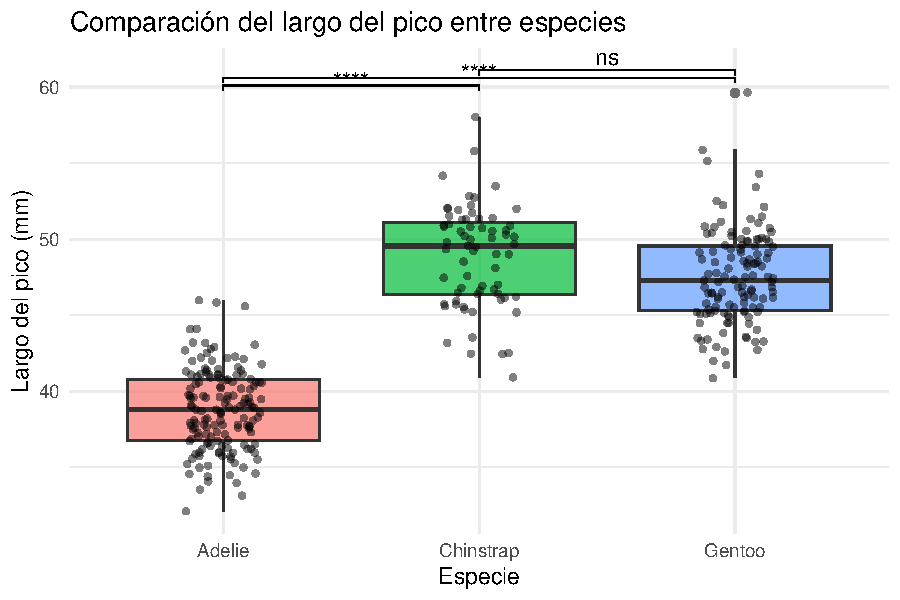
\includegraphics[keepaspectratio]{Prueba-de-hipótesis_files/figure-pdf/boxplot_kruskal-1.pdf}}

}

\caption{Boxplot de bill\_length\_mm por especie con comparaciones
post-hoc (Dunn).}

\end{figure}%

La \textbf{Figura 1} muestra la distribución del largo del pico en las
tres especies de pingüinos (\emph{Adelie}, \emph{Chinstrap} y
\emph{Gentoo}). Se observa que los \emph{Adelie} presentan valores
menores y más concentrados (mediana cercana a 38--40 mm), mientras que
los \emph{Chinstrap} tienen los picos más largos (mediana en torno a
48--50 mm). Los \emph{Gentoo} ocupan una posición intermedia, con
valores cercanos a 46--48 mm y mayor variabilidad en comparación con
\emph{Adelie}.

Las comparaciones post-hoc de Dunn con corrección de Bonferroni
evidencian diferencias altamente significativas en \emph{Adelie vs
Chinstrap} (****) y \emph{Adelie vs Gentoo} (****\emph{).} Por el
contrario, no se encontraron diferencias significativas entre
\emph{Chinstrap} vs \emph{Gentoo} (ns).

\section{Conclusiones generales}\label{conclusiones-generales}

\begin{itemize}
\item
  El análisis estadístico mediante Kruskal--Wallis confirmó diferencias
  significativas en la distribución del largo del pico entre especies de
  pingüinos (χ² = 244.1, p \textless{} 0.001), con un tamaño de efecto
  muy grande (ε² = 0.71). Esto indica que la especie explica una
  proporción sustancial de la variabilidad observada en la morfología
  del pico.
\item
  Las pruebas post-hoc mostraron que los \emph{Adelie} difieren
  significativamente de \emph{Chinstrap} y \emph{Gentoo}, mientras que
  estas dos últimas no presentan diferencias estadísticamente
  significativas entre sí.
\item
  Desde una perspectiva ecológica, los resultados sugieren que
  \emph{Adelie} ocupa un nicho trófico diferenciado, asociado al consumo
  de krill y pequeños invertebrados, lo que reduce la competencia
  directa con las otras especies. En cambio, \emph{Gentoo} y
  \emph{Chinstrap}, al presentar longitudes de pico más similares,
  podrían solaparse en el aprovechamiento de presas de mayor tamaño
  (peces e invertebrados grandes).
\item
  En conjunto, los hallazgos respaldan la hipótesis de una segregación
  morfológica y trófica que favorece la coexistencia de las tres
  especies en el ecosistema antártico.
\end{itemize}

\section{Anova con transformación
logarítmica}\label{anova-con-transformaciuxf3n-logaruxedtmica}

\begin{Shaded}
\begin{Highlighting}[numbers=left,,]
\NormalTok{df }\OtherTok{\textless{}{-}}\NormalTok{ df }\SpecialCharTok{\%\textgreater{}\%}
  \FunctionTok{mutate}\NormalTok{(}\AttributeTok{log\_bill\_length =} \FunctionTok{log}\NormalTok{(bill\_length\_mm))}

\NormalTok{modelo\_log }\OtherTok{\textless{}{-}} \FunctionTok{aov}\NormalTok{(log\_bill\_length }\SpecialCharTok{\textasciitilde{}}\NormalTok{ species, }\AttributeTok{data =}\NormalTok{ df)}

\CommentTok{\# Supuestos}
\NormalTok{shapiro\_res }\OtherTok{\textless{}{-}} \FunctionTok{shapiro.test}\NormalTok{(}\FunctionTok{residuals}\NormalTok{(modelo\_log))}
\NormalTok{levene\_res  }\OtherTok{\textless{}{-}} \FunctionTok{leveneTest}\NormalTok{(log\_bill\_length }\SpecialCharTok{\textasciitilde{}}\NormalTok{ species, }\AttributeTok{data =}\NormalTok{ df)}

\CommentTok{\# Tablas}
\NormalTok{knitr}\SpecialCharTok{::}\FunctionTok{kable}\NormalTok{(}
\NormalTok{  broom}\SpecialCharTok{::}\FunctionTok{tidy}\NormalTok{(shapiro\_res),}
  \AttributeTok{caption =} \StringTok{"Test de normalidad de residuos (Shapiro{-}Wilk)"}
\NormalTok{)}
\end{Highlighting}
\end{Shaded}

\begin{longtable}[]{@{}rrl@{}}
\caption{Test de normalidad de residuos (Shapiro-Wilk)}\tabularnewline
\toprule\noalign{}
statistic & p.value & method \\
\midrule\noalign{}
\endfirsthead
\toprule\noalign{}
statistic & p.value & method \\
\midrule\noalign{}
\endhead
\bottomrule\noalign{}
\endlastfoot
0.9945676 & 0.2675526 & Shapiro-Wilk normality test \\
\end{longtable}

\begin{Shaded}
\begin{Highlighting}[numbers=left,,]
\NormalTok{knitr}\SpecialCharTok{::}\FunctionTok{kable}\NormalTok{(}
\NormalTok{  broom}\SpecialCharTok{::}\FunctionTok{tidy}\NormalTok{(levene\_res),}
  \AttributeTok{caption =} \StringTok{"Test de homogeneidad de varianzas (Levene)"}
\NormalTok{)}
\end{Highlighting}
\end{Shaded}

\begin{longtable}[]{@{}rrrr@{}}
\caption{Test de homogeneidad de varianzas (Levene)}\tabularnewline
\toprule\noalign{}
statistic & p.value & df & df.residual \\
\midrule\noalign{}
\endfirsthead
\toprule\noalign{}
statistic & p.value & df & df.residual \\
\midrule\noalign{}
\endhead
\bottomrule\noalign{}
\endlastfoot
0.5610386 & 0.571145 & 2 & 339 \\
\end{longtable}

\begin{Shaded}
\begin{Highlighting}[numbers=left,,]
\CommentTok{\#|label: anova}
\NormalTok{Anova\_res }\OtherTok{\textless{}{-}} \FunctionTok{summary}\NormalTok{(modelo\_log)}
\NormalTok{Anova\_res}
\end{Highlighting}
\end{Shaded}

\begin{verbatim}
             Df Sum Sq Mean Sq F value Pr(>F)    
species       2  3.846  1.9230   427.6 <2e-16 ***
Residuals   339  1.525  0.0045                   
---
Signif. codes:  0 '***' 0.001 '**' 0.01 '*' 0.05 '.' 0.1 ' ' 1
\end{verbatim}

En la \textbf{Tabla 4} se presentan los resultados de la prueba de Anova
(log-transformado): F = , gl = 2, p = . El valor p es mucho menor a
0.05, lo que indica diferencias altamente significativas en el largo del
pico entre las tres especies de pingüinos.

\section{Comparaciones post-hoc (Tukey
HSD)}\label{comparaciones-post-hoc-tukey-hsd}

\begin{Shaded}
\begin{Highlighting}[numbers=left,,]
\CommentTok{\#|label: Post{-}hoc de Tukey}

\NormalTok{tukey\_res }\OtherTok{\textless{}{-}} \FunctionTok{TukeyHSD}\NormalTok{(modelo\_log)}
\NormalTok{tukey\_res}
\end{Highlighting}
\end{Shaded}

\begin{verbatim}
  Tukey multiple comparisons of means
    95% family-wise confidence level

Fit: aov(formula = log_bill_length ~ species, data = df)

$species
                        diff         lwr          upr    p adj
Chinstrap-Adelie  0.23023589  0.20718014  0.253291643 0.000000
Gentoo-Adelie     0.20292758  0.18375262  0.222102538 0.000000
Gentoo-Chinstrap -0.02730831 -0.05116498 -0.003451639 0.020178
\end{verbatim}

En la \textbf{Tabla 5} se presentan las comparaciones por pares (Tukey
HSD):

\begin{itemize}
\item
  \emph{Adelie} vs \emph{Chinstrap}: p.adj = → diferencia significativa.
\item
  \emph{Adelie} vs \emph{Gentoo}: p.adj = → diferencia significativa.
\item
  \emph{Chinstrap} vs \emph{Gentoo}: p.adj = → diferencia significativa,
  aunque de magnitud mucho menor que en los otros contrastes.
\end{itemize}

Las comparaciones muestran que el largo del pico en \emph{Adelie}
difiere significativamente tanto de \emph{Chinstrap} como de
\emph{Gentoo}. Mientras que entre \emph{Chinstrap} y \emph{Gentoo} no se
detectan diferencias estadísticamente significativas en el largo del
pico. Esto sugiere que la dieta de \emph{Adelie} es distinta a la de las
otras especies. Mientras que entre \emph{Gentoo} y \emph{Chinstrap},
podrían compartir parcialmente los mismos recursos tróficos. En
conjunto, la prueba confirma una clara segregación de \emph{Adelie}
respecto a las otras especies, lo que reduce la competencia y favorece
la coexistencia de las tres especies en el ecosistema antártico.

\section{Conclusiones generales}\label{conclusiones-generales-1}

\begin{itemize}
\item
  El ANOVA transformado confirma que el largo del pico difiere
  significativamente entre las tres especies de pingüinos.
\item
  \emph{Adelie} presenta picos claramente más cortos que
  \emph{Chinstrap} y \emph{Gentoo}, lo cual concuerda con su
  especialización en krill y pequeños invertebrados.
\item
  \emph{Chinstrap} posee picos más largos, asociados a una dieta más
  flexible (peces e invertebrados de mayor tamaño).
\item
  \emph{Gentoo}, aunque intermedio, muestra diferencias significativas
  con ambas especies: picos más largos que \emph{Adelie} y ligeramente
  más cortos que \emph{Chinstrap}.
\item
  En conjunto, los resultados sugieren una segregación trófica clara de
  \emph{Adelie}, mientras que Gentoo y \emph{Chinstrap} solapan
  parcialmente en el uso de recursos, pero aun así presentan diferencias
  detectables estadísticamente.
\end{itemize}




\end{document}
